%%%%%%%%%%%%%%%%%%%%%%%%%%%%%%%%%%%%%%%%%%%%%%%%%%%%%%%%%%%%%%%%%%%%%%
% Problem statement
\begin{statement}[
  problempoints=100,
  timelimit=1 sekunda,
  memorylimit=512 MiB,
]{Kraljevstvo}

Jednom davno, u ona davna, davna vremena, na ovim je prostorima postojalo
veliko i bogato kraljevstvo koje se sastojalo od $N$ dvoraca u kojima su živjeli
mještani. Zanimljivo je da kraljevstvom nije vladao jedan, već dva kralja.
Kralj Istok živio je u najistočnijem dvorcu, dok je kralj Zapad živio u
najzapadnijem. Nažalost, idiličan život mještana prekinula je vijest o
razbojničkoj bandi koja juri prema kraljevstvu.

Vremena je sve manje, a kraljevstvo nije moguće u potpunosti zaštititi bez
poduzimanja drastičnih mjera. Teška srca, kraljevi će odabrati točno $K$
dvoraca koje će dodatno osnažiti selidbom stanovnika iz preostalih $N - K$
dvoraca. Naravno, među $K$ osnaženih dvoraca nalazit će se i dvorci u kojima
oni sami žive.  Također, osnažene će dvorce ograditi zidinama tako da one
tvore \textit{konveksnu ljusku} tog skupa dvoraca. Primijetite da se prazni
dvorci mogu, ali i ne moraju nalaziti unutar te konveksne ljuske.

Logično, kraljevi su odlučili osnažiti $K$ dvoraca tako da površina zidinama
ograđenog dijela bude najveća moguća. Odredite tu površinu.

\textbf{Napomena:} konveksna ljuska nekog skupa točaka odgovara konveksnom
poligonu najmanje površine koji sadrži (na svojim bridovima, vrhovima ili
u unutrašnjosti) sve točke tog skupa.

%%%%%%%%%%%%%%%%%%%%%%%%%%%%%%%%%%%%%%%%%%%%%%%%%%%%%%%%%%%%%%%%%%%%%%
% Input
\subsection*{Ulazni podaci}
U prvom su retku prirodni brojevi $N$ i $K$ $(3 \le K \le N)$ iz teksta zadatka.

U $i$-tom od sljedećih $N$ redaka nalaze se po dva broja $x_i$ i $y_i$ $(0 \leq
|x_i|, |y_i| \leq 10^9)$ koji označavaju da se $i$-ti dvorac u koordinatnoj
ravnini nalazi na poziciji $(x_i, y_i)$. Pritom se niti jedan par dvoraca neće
nalaziti na istoj poziciji.

Također, prvi od navedenih dvoraca odgovara dvorcu kralja Zapada $(y_1 = 0, x_1
< x_i, i \ne 1)$, dok drugi navedeni dvorac odgovara dvorcu kralja Istoka
$(y_2 = 0, x_2 > x_i, i \ne 2)$. Primijetite da oba dvorca leže na $x$-osi.

%%%%%%%%%%%%%%%%%%%%%%%%%%%%%%%%%%%%%%%%%%%%%%%%%%%%%%%%%%%%%%%%%%%%%%
% Output
\subsection*{Izlazni podaci}
U jedini je redak potrebno ispisati realan broj koji predstavlja traženu
površinu iz teksta zadatka.

Površinu treba ispisati bez vodećih i pratećih nula. Primjerice, ako je
tražena površina iznosi $3.14$, ispisi poput $03.14$ ili $3.1400$ neće
se priznavati.

%%%%%%%%%%%%%%%%%%%%%%%%%%%%%%%%%%%%%%%%%%%%%%%%%%%%%%%%%%%%%%%%%%%%%%
% Scoring
\subsection*{Bodovanje}
{\renewcommand{\arraystretch}{1.4}
  \setlength{\tabcolsep}{6pt}
  \begin{tabular}{ccl}
 Podzadatak & Broj bodova & Ograničenja \\ \midrule
  1 & 11 & $3 \le N \le 20$ \\
  2 & 25 & $3 \le N \le 100$ \\
  3 & 15 & $3 \le N \le 500$ \\
  4 & 49 & $3 \le N \le 3\,000$ \\
\end{tabular}}

%%%%%%%%%%%%%%%%%%%%%%%%%%%%%%%%%%%%%%%%%%%%%%%%%%%%%%%%%%%%%%%%%%%%%%
% Examples
\subsection*{Probni primjeri}
\begin{tabularx}{\textwidth}{X'X'X}
\sampleinputs{test/kraljevstvo.dummy.in.1}{test/kraljevstvo.dummy.out.1} &
\sampleinputs{test/kraljevstvo.dummy.in.2}{test/kraljevstvo.dummy.out.2} &
\sampleinputs{test/kraljevstvo.dummy.in.3}{test/kraljevstvo.dummy.out.3}
\end{tabularx}

\textbf{Pojašnjenje prvog probnog primjera:}
Optimalno je osnažiti dvorce na pozicijama $(0,0)$, $(2, -7)$, $(2, 8)$ i $(9, 0)$
kao što je prikazano na lijevoj skici.

\textbf{Pojašnjenje drugog probnog primjera:}
Optimalno je osnažiti dvorce na pozicijama $(0,0)$, $(10, 0)$ i $(5, -5)$
kao što je prikazano na desnoj skici.

\begin{figure}[H]
\centering
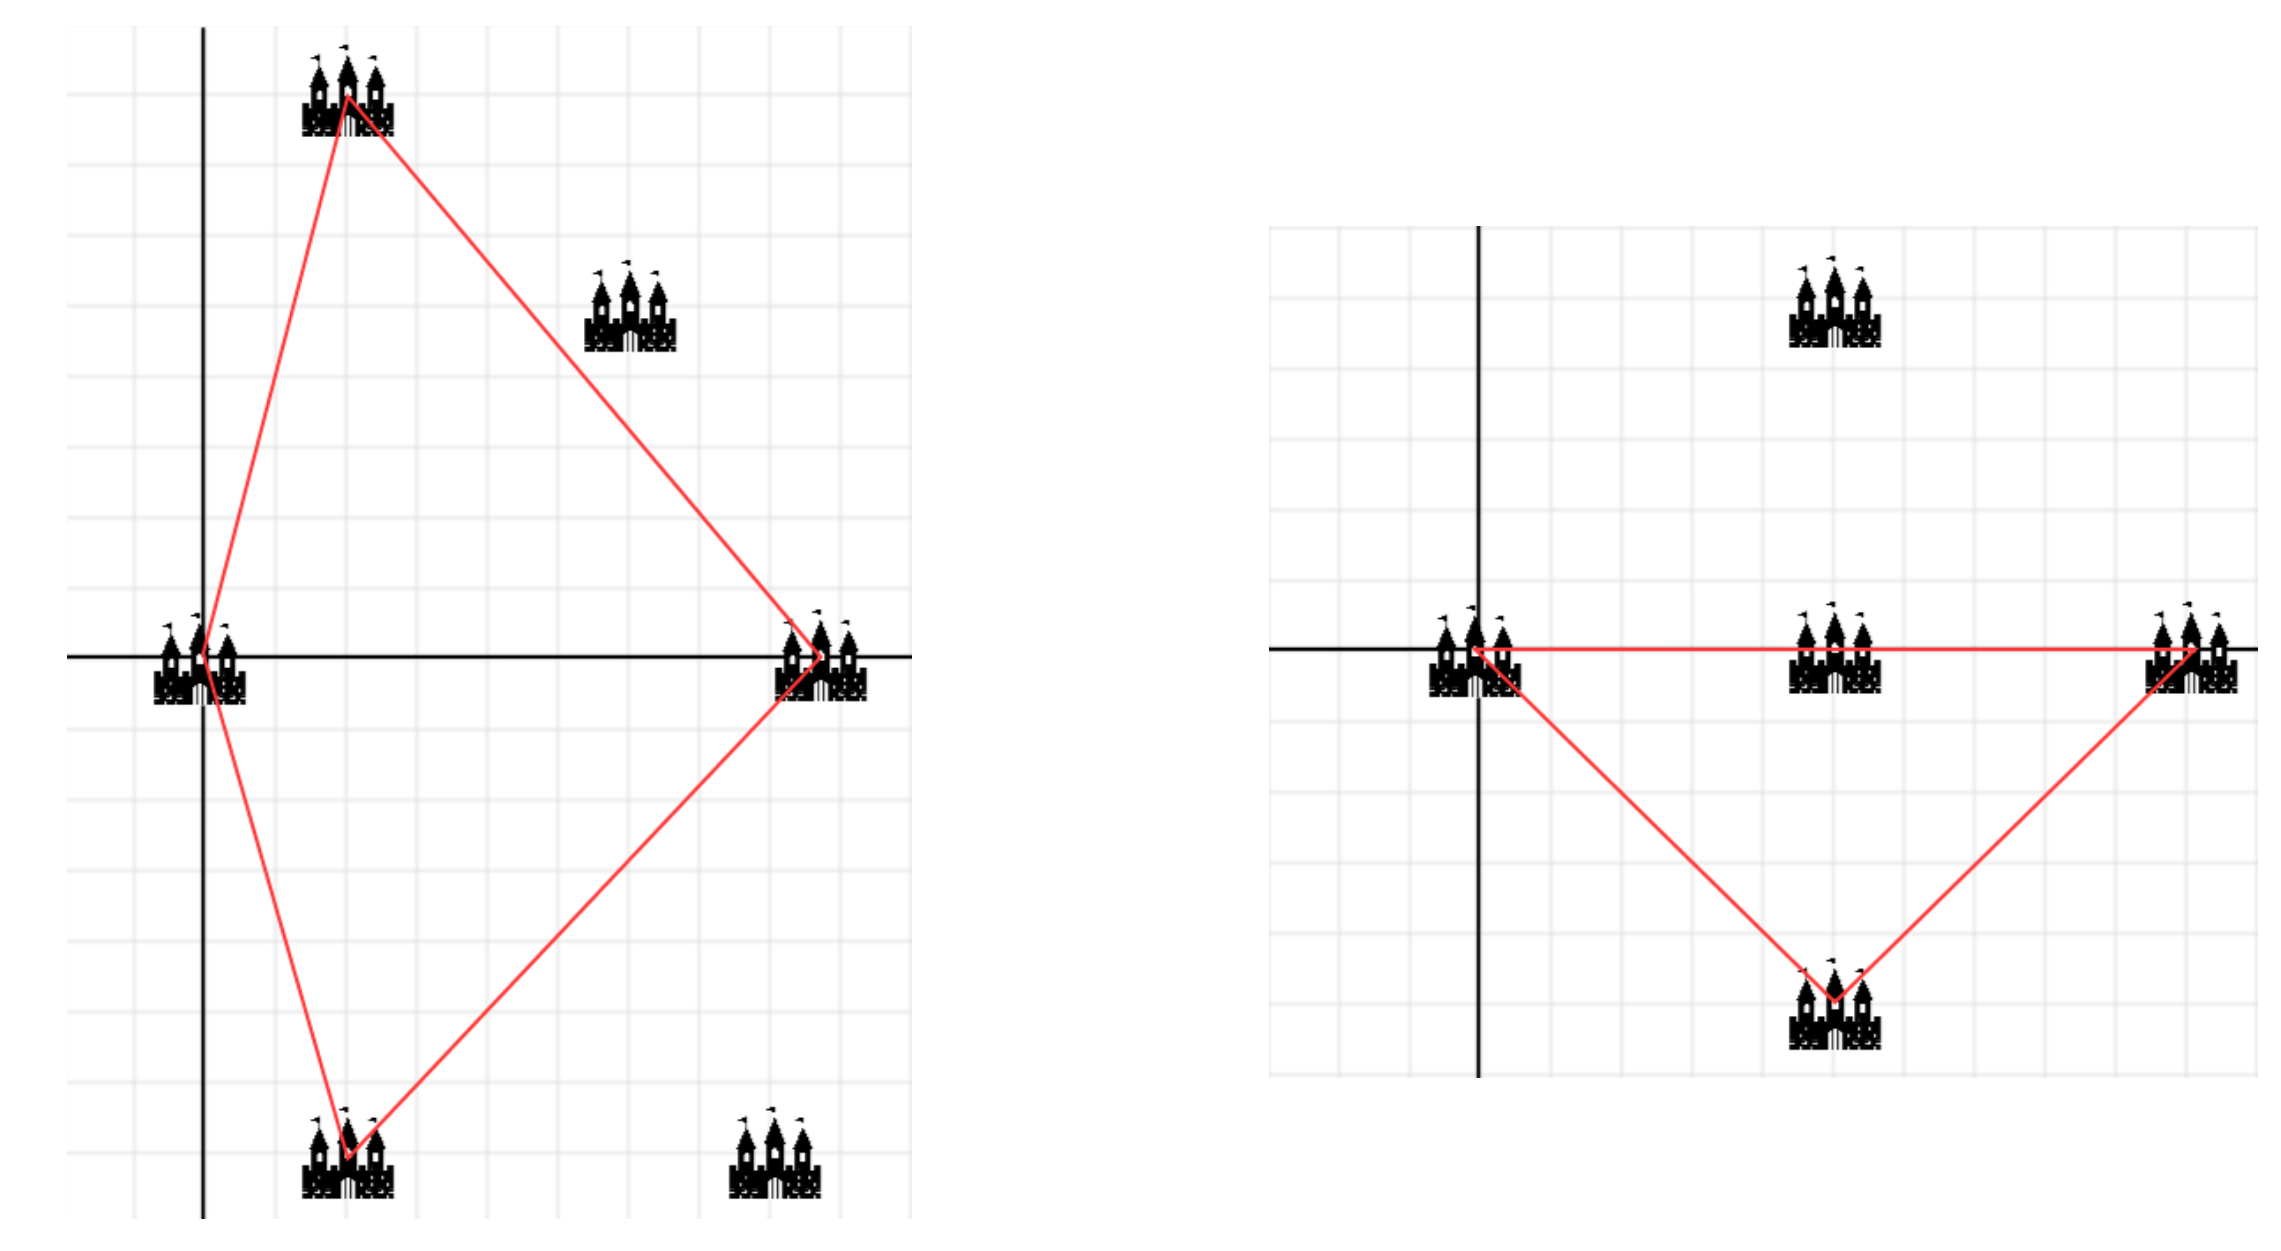
\includegraphics[width=\textwidth]{img/dummy_skice.png}
\end{figure}


%%%%%%%%%%%%%%%%%%%%%%%%%%%%%%%%%%%%%%%%%%%%%%%%%%%%%%%%%%%%%%%%%%%%%%
% We're done
\end{statement}

%%% Local Variables:
%%% mode: latex
%%% mode: flyspell
%%% ispell-local-dictionary: "croatian"
%%% TeX-master: "../hio.tex"
%%% End:
